\documentclass[final,12p,times]{elsarticle}
\usepackage[noprefix]{nomencl}
\usepackage{times}
\usepackage{graphicx}
\usepackage{float}
%\usepackage{enumerate}
\usepackage{amssymb}
\usepackage{enumitem}
\usepackage{array}
\usepackage[ruled]{algorithm2e}
\usepackage{hyperref}
\providecommand{\SetAlgoLined}{\SetLine}
\renewcommand{\nomname}{List of Abbreviations}
\renewcommand{\figurename}{Fig.}
\floatstyle{ruled}
\journal{Machine Learning Engineer Nanodegree}
\begin{document}
\begin{frontmatter}
\title{Using Deep Neural Networks for Object Detection in Images: A Paradigm Using the Google SVHN Dataset}
\author[rvt]{Avraam Th. Tolmidis\corref{cor1}}
\ead{atolmid@gmail.com}


\begin{keyword}
Deep Learning \sep Image recognition \sep Convolutional Neural Networks 
\end{keyword}
\end{frontmatter}
\makenomenclature

\section{Scope}
In this document, the results of the Deep Learning Capstone Project of the Udacity Machine Learning Nanodegree will be presented.
The aim of the project was to select a field where the knowledge acquired during the Nanodegree can be used to solve a real-world problem.
The interest of the author was primarily Deep Learning, thus the project described was selected.
The specific problem has been studied in the past, its current study however, provides hands-on experience with a real-world problem, 
and promotes deeper understanding of the topic.
In addition, the specific project choice builds the foundations for working later on more complex and novel applications.
%\end{Proposal}

\section{Introduction}
\label{Intro}
The problem of identifying digits from street images is still considered an open problem.
In the recent years there have been advances, mostly due to the use of Deep Learning architectures.
Deep learning is a field in Artificial Intelligence that emerged during the recent years, building on the concept of Neural Networks.
Neural networks in principle try to emulate the information processing capabilities of human neurons.
They try to process complex data, and are used for both regression, as well as classification problems. 
However, due to the large number of computations that are required, there were limitations on the use of Neural Networks on large-scale 
problems, as it was not possible to use networks with many layers.
%An overview of Deep Learning Methods and Applications can be found in \cite{deep-learning-methods-and-applications}.
As more efficient hardware became recently available, capable of performing large amounts of calculations, the use of Deep Neural Networks 
for solving difficult problems, such as the Image Recognition studied in the present, became more common.
Image recognition using Deep Neural Networks yields an accuracy comparable to that achieved by humans, e.g. 97.84\% (per-digit identification in images) \cite{DBLP:journals/corr/GoodfellowBIAS13}.


\section{Object Detection in Images}
\label{sec:1}
Object detection in images and videos, or their classification, is very important lately, as they enable a plethora of applications.
It includes detecting objects and recognising patterns in sequential images/video frames. 
The use of such applications, and the demand for them has increased significantly during the last years, for many reasons, including:
\begin{itemize}
\item The massive use of cameras (including their integration in mobile phones), that makes endless sources of image and video available.
\item The availability of more efficient hardware than in the past, capable of processing big amounts of data.
\item The use of new/refined image processing techniques.
\end{itemize}

Some of the most common methods that have been used so far for this purpose are described in the following paragraphs.

\emph{Optical Flow} \cite{chauhan2013moving} calculates the optical flow field of an image. Then, using the optical flow distribution characteristics of 
the image, it performs clustering. It is used for distinguishing a moving object from the background, achieving a relatively high accuracy.
However, it is not considered a method suitable for real-time object detection, since a lot of calculations are required, and it is additionally 
sensitive to noise.

\emph{Point detectors} try to find points in images that have distinct characteristics, relevant to their locality \cite{lee2009histogram} \cite{rout2013survey}. They are 
points that do not get affected by changes in the point where the image was taken from, or illumination

In \emph{Background Subtraction} we work with video images. Implementing the method, we follow in principle the 
following steps: We construct a representation of the background model, and look for deviations stemming
from the model for each next frame in the video. If there is a change in a part of the image that is noteworthy, we consider this as a 
moving object. The pixels this image region consists of, are then processed further.
There are two types of algorithms, \emph{Recursive}, and \emph{Non-recursive}.

\begin{itemize}
\item \emph{Recursive Algorithms} \cite{sen2004robust} \cite{srinivasan2009improved} update a single background model, based on each input frame. Since they do not use a buffer, 
they require less storage than non-recursive techniques. However, the model is influenced by images that extend to the more distant past, 
and this means that any errors in the model are propagated to future instances.

\item \emph{Non-Recursive Algorithms} \cite{sen2004robust} \cite{srinivasan2009improved} on the other hand, use storage, whose requirements can sometimes be high, however, 
they are immune to the influence of frames that extend deeply in the past.
A buffer is stored, that contains The L previous frames.
By considering the changes in the frames of the buffer with time, an estimation of the image is performed.
A common method is \emph{Simple Background Subtraction} \cite{rout2013survey} \cite{kim2002fast} \cite{zhan2007improved}, where we try to find a motion detection mask D.
In order to do this, we take the absolute difference between the current image, and a reference background image, which is usually the 
first frame of the video, without containing any foreground objects.
\end{itemize}

\emph{Frame differencing} \cite{rakibe2013background} detects moving objects by calculating the difference between two consecutive images.
 
\emph{Temporal differencing} \cite{joshi2012survey} on the other hand, detects moving regions by examining the pixel-wise difference between two or 
three frames in a video. It is a relatively effective method, with a somewhat lower effectiveness though, when the object moves slowly, 
or its texture is uniform \cite{paragios2000geodesic} \cite{zhu1996region}.  The object is no longer detected when it stops moving, since there is no difference between the 
consecutive frames.

For a more detailed study of Object detection in Images, the reader can refer to \cite{bushrasurvey}

\section{Deep Neural Networks for Image Object Recognition}
\label{sec:2}
In the present work we study the use of Deep Learning models in order to decode sequences of digits from natural images.
Deep Neural Networks are used lately more often in object detection, due to their characteristics, which prove very convenient.
In principle, we do not need to define specific features in order to detect objects and classify them.
This will be performed by the network itself, through the update of the weights of the connections between the network layers.

The most limiting factor until recently was the restriction with regards to the number of layers and nodes that could be used.
The large amount of computations required, was making it impossible to use more than a few number of layers.
The evolution of the available hardware though, and the use of GPUs capable of performing a large number of computations per second, 
enabled the use of many more layers, up to tens of them.
Furthermore, the growing availability of large datasets provides the conditions to train neural networks with a larger amount of data, 
hence improving their accuracy.
Additionally, the use of concepts like \emph{Convolutional Neural Networks} \cite{Fukushima1980} \cite{Lecun98gradient-basedlearning}, 
improve the accuracy of the detection to a level comparable with the capabilities of a human.

A \emph{Neural Network}, consists of layers of \emph{neurons}.
A single neuron can be seen in figure \ref{fig:Fig2.1}

\begin{figure}[H]
%\begin{center}
  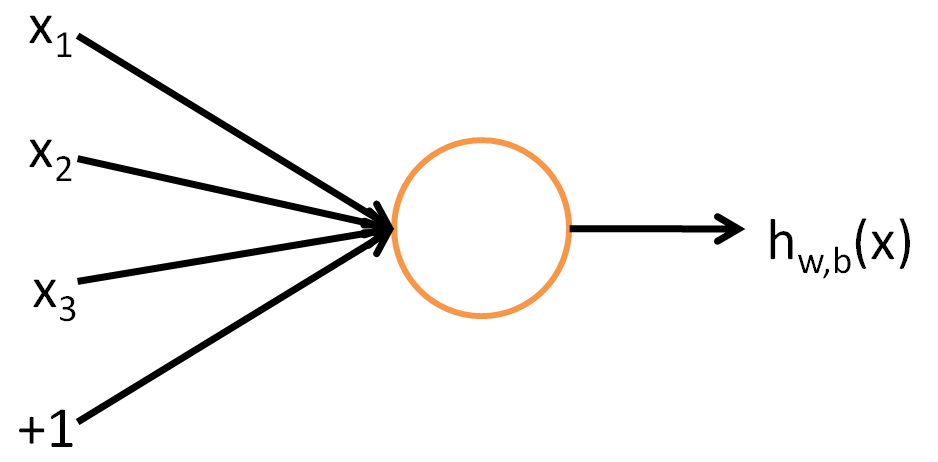
\includegraphics[width=1.0\textwidth, center]{SingleNeuron.png}
%  \end{center}
  \caption{A single neuron}
  \label{fig:Fig2.1}
  \end{figure}
  
The neuron has a number of inputs (x1,x2,x3,...) as well as an additional intercept term.
Its output is \begin{math} h_{W,b}(x) = f(W^Tx) = f(\sum_{i=1}^3 W_{i}x_i +b)\end{math}, 
and it's called the \emph{Activation Function}
Common activation function choices are the \emph{sigmoid function}:


\begin{math}f(z) = \frac{1}{1+\exp(-z)}\end{math}

or, the tanh, function:


\begin{math}f(z) = \tanh(z) = \frac{e^z - e^{-z}}{e^z + e^{-z}}\end{math}, 
 

The tanh(z) function gives us the opportunity to have a function that has an output range centred at zero, since its output range is [−1,1] instead of [0,1] that the sigmoid has.

Thus, the neural network is in principle a combination of layers of nodes, which can have multiple inputs, as well as multiple outputs.
These layers are the \emph{fully connected layers} - or the \emph{feed forward neural network}.
An example of a simple neural network is presented in figure \ref{fig:Fig2.2}

\begin{figure}[H]
%\begin{center}
  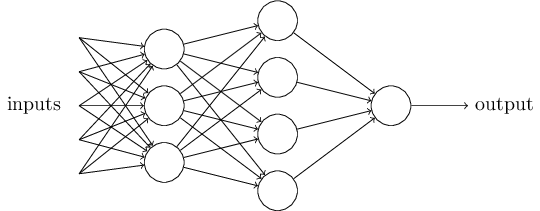
\includegraphics[width=1.0\textwidth, center]{NN.png}
%  \end{center}
  \caption{A single neuron}
  \label{fig:Fig2.2}
  \end{figure}


A \emph{Convolutional Neural Network (CNN)} is a network that can contain several functions, like convolution, pooling, non-linear functions, normalisation and fully connected layers. 
In most cases, there are convolutional layers, that are followed by normal, fully connected layers, like the ones described above.

CNNs are mostly used for image recognition, and each of their layers acts in practice as a filter, detecting specific features, or patterns.
The first layers detect simplest features such as lines or curves, while each consecutive layer detects more abstract features, that may combine features from the previous layers.
Using the data from the previous layers, the last layer is usually used in order to perform a classification task.

Each Convolution layer of the has a specific filter, which is able to detect features in the image, regardless of the position of the feature in the image.
The filter is applied on the image data, and shifted multiple times, until it has been over the whole image. 
For the image that is represented as a matrix of pixel values, the filter will be a matrix of a smaller dimension (usually 3x3 or 5x5), 
Following at least one of the convolution layers, is usually a pooling operation, where the filter slides over the image data matrix by a number of pixels (called the \emph{stride}).
An element wise multiplication is performed between the two matrices, and the outputs are then added, and they provide the elements of the (final) output matrix or \emph{Activation Map}.
The Convolutional layers are common, meaning the same parameters are shared by all features.
A visualisation of the above process can be seen in figure \ref{fig:Fig2.3}.

\begin{figure}[H]
%\begin{center}
  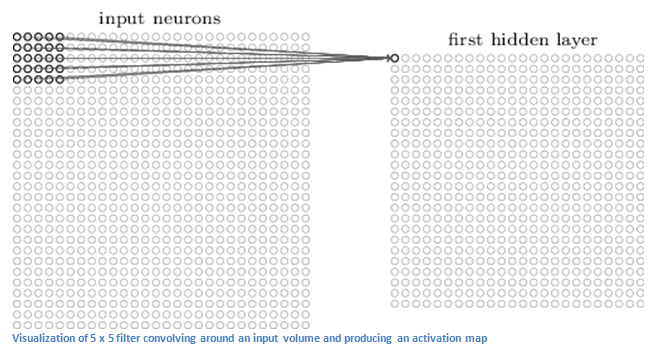
\includegraphics[width=1.0\textwidth, center]{ActivationMap.png}
%  \end{center}
  \caption{Activation Map Creation Process}
  \label{fig:Fig2.3}
  \end{figure}

A commonly used function to introduce non-linearity to the model is the \emph{Rectified Linear Unit (ReLU)}.
It is usually used after each convolution, and provides as output the maximum between its input, and zero.
the operation can be seen in figure \ref{fig:Fig2.4}.
\begin{figure}[H]
%\begin{center}
  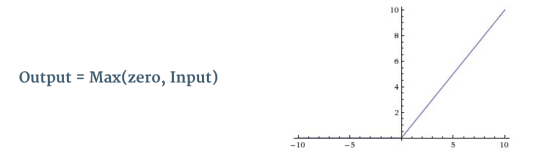
\includegraphics[width=1.0\textwidth, center]{relu.png}
%  \end{center}
  \caption{ReLU Operation}
  \label{fig:Fig2.4}
  \end{figure}
 

  
The pooling, or \emph{subsampling} function, is used to reduce the dimensionality of the data.
There are different types of pooling operations, such as sum, max, average, etc.
In principle, neighbouring elements in a matrix are summarized to one element in a new matrix, of lower dimensions.
The new dimension is chosen as part of the model design, as well as what will be the pooling operation used.
A Max Pooling operation is displayed in figure \ref{fig:Fig2.5}, which is taken from the material of the Stanford 
\emph{CS231n: Convolutional Neural Networks for Visual Recognition} course.

\begin{figure}[H]
%\begin{center}
  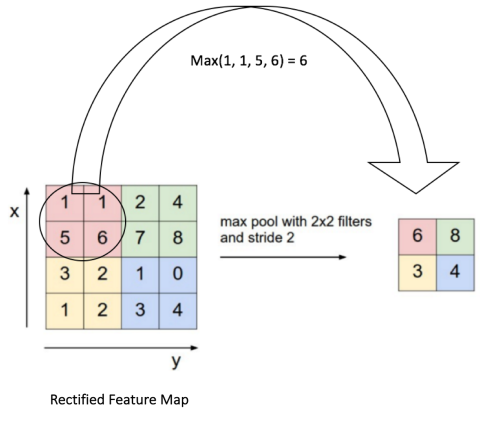
\includegraphics[width=1.0\textwidth, center]{pooling.png}
%  \end{center}
  \caption{A Max Pooling Operation}
  \label{fig:Fig2.5}
  \end{figure}


To avoid the effect of \emph{overfitting} the data (learning to recognise the data used to train the network, but failing to accurately predict new data), there are several methods used,
one of which in specific (that will also be a subject of study in the present work) is \emph{dropout} \cite{Srivastava2014}.
With dropout, a percentage of the inputs to each neuron in a layer that it is applied, is randomly ignored.
This results in higher accuracy levels when classifying new data, in the case where overfitting occurs.
However, the network then requires more training, otherwise the desired result might not be achieved.

An example of a Neural Network with convolution layers is shown in figure \ref{fig:Fig2.6}, where the LeNet network is presented \cite{Lecun98gradient-basedlearning}.
There are two Convolution layers, each followed by \emph{max-pooling}, with two fully-connected layers, that provide the outputs.

\begin{figure}[H]
%\begin{center}
  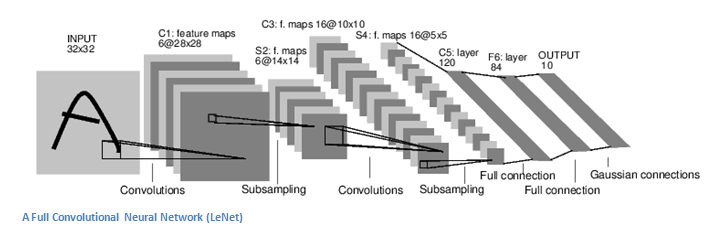
\includegraphics[width=1.0\textwidth, center]{LeNet.png}
%  \end{center}
  \caption{The LeNet Architecture}
  \label{fig:Fig2.6}
  \end{figure}


\section{Project Overview}
\subsection{Problem Statement}
\label{sec:3.1}
The purpose of this work is to study the behaviour of Deep Learning models when used in order to decode sequences of digits from natural 
images.
For this task, Convolutional Neural Networks were used. 

The work consists of two individual sections:
\begin{Itemize}
\item Initially, the effort was not to predict individual digits, \emph{but the complete house number}, when using as input the 
part of the image that co tains the numbers.
The numbers consist of 1, to 5 digits for the biggest.
In order to make the implementation easier, all numbers were considered having the maximum amount of digits (5).
When the numbers consisted of less than 5 digits, padding was used, in order to add the missing digits in the 
beginning of the number.
Since - as we will see below - the constructors of the dataset used for the labels digits 1 to 9 to represent one to nine,
and the number 10 to represent zero, 0 was selected to represent "digit does not exist".
For example, a number 11, in order to have five digits, was turned to 00011, 2317 changed to 02317, etc.

The behaviour/performance of the model was studied, with different network parameters (optimizer, techniques like dropout, 
etc.).
It was compared to the naive approach where we only have a simple regression with a Gradient Descent optimizer. 
The implementation of the project was a Python application, using different Python scripts for independent parts of the 
application.
\item The second part was attempting to recognise just the individual digits. for this purpose, a second dataset was used, where
the digits have already been separated.
In this case the problem solution was simpler, since there was no need considering the length of a number (always one digit).
Therefore, the model was significantly simplified, as well the way of estimating prediction accuracy.
Additionally, the preprocessing of the data was significantly required.
 
\subsection{Evaluation Metrics}
\label{sec:3.2}

As already mentioned, the evaluation metric was the detection accuracy.
In the case where the complete number has to be recognised, the accuracy was evaluated as shown in Algorithm \ref{alg1}:


\begin{algorithm}[H]
 \SetAlgoLined
 \For {all digits i}{
    prediction:
	\begin{math}p[i] $=$ argmax(predictions)\end{math}\;
  	label:
  	\begin{math}l[i] $=$ argmax(labels)\end{math}\;}
  \For {every image} {
	successful digits $=$ sum(p[i] $=$$=$ l[i])}
	   
   \begin{math}accuracy(\%) $=$ 100 * count(successful digits $=$ $=$ 5) / number of images\end{math}
\caption{Estimation of accuracy \%}
\label{alg1}
\end{algorithm}


The number is correctly identified only when all five digits (including any zeros used for padding in the beginning of the 
number) have been identified.
This means, for example, that for the number 11, the two digits have been successfully identified, and three zeros have been 
added in front of them (00011).
The percentage of all images, for which all five digits were correctly identified gives us the accuracy.

In the second part, since each time we need to recognise one digit, accuracy estimation is much simpler:
it is the percentage of digits that have been correctly identified.

Since the digits dataset is not a balanced one (see subsection \ref{sec:4.1}), the choice of a metric such as the F1 score 
would probably be a better choice.
However, since most work that can be used as a baseline for comparison uses accuracy, accuracy was also the choice here, in 
order to make it easier to compare results.
In the case of the first part of the work, where the complete sequence of digits has to be correctly identified in order to 
get a correct prediction, using the F1 score would additionally require more complex, custom functions, to be developed.

\section{Analysis}
\subsection{Data Exporation and Visualisation}
\label{sec:4.1}
The data that used was that from the Google Street View House Number dataset \cite{ 37648}. 
SVHN is a real-world image dataset for developing machine learning and object recognition algorithms. 
The images are coloured, and consist of small digits (over 600,000), from natural scene images. 
The dataset is obtained from house numbers in Google Street View images.

There are - as already mentioned - two distinct datasets:
One that contains complete numbers (used during the first part of this work), and one that contains images of individual digits.
For simplicity we will refer to the first dataset as "numbers" dataset, and to the second one as "digits" dataset.

In the numbers dataset, an issue with the images in the dataset is that they are not all the same size.
Images vary in size, for example 54x21 (image 101 of the training set), 176x92 (image 99 of the training set), or larger, such 
as image 100 of the training set, which is 353x133.
Depending on the process used to detect and identify the content, this can be a problem during the development of the algorithm.
To mitigate this issue, during the preprocessing phase, the output of the images was resized: 
All images, after preprocessing, have a size of 128x128.
More details on the preprocessing of the images can be found in chapter \ref{sec:5}.

The numbers dataset contains 10 classes, 1 for each digit. 
Digit '1' has label 1, '9' has label 9 and '0' has label 10.
The maximum number length is considered to consist of 5 digits. 
Since in the first part the goal is to identify complete numbers and not separate digits, the varying length is problem.
Therefore, to make things simpler, the number of digits is considered fixed, and 5. 
To account for the numbers of smaller length, an additional class with label 0 was added to the dataset. 
It represents the digits that need to be added in the front of the number, in order to make its length equal to 5.
As already mentioned, this means that the number 11, for example, would have the label 00011.
Thus, all labels in the numbers dataset, after preprocessing have a length of 5.
Each of the digits in the labels is finally  one-hot-encoded, with 11 classes (one for the "no-digit" case).
An example of SVHN images can be seen in figure \ref{fig:Fig4.1}.

\begin{figure}[H]
%\begin{center}
  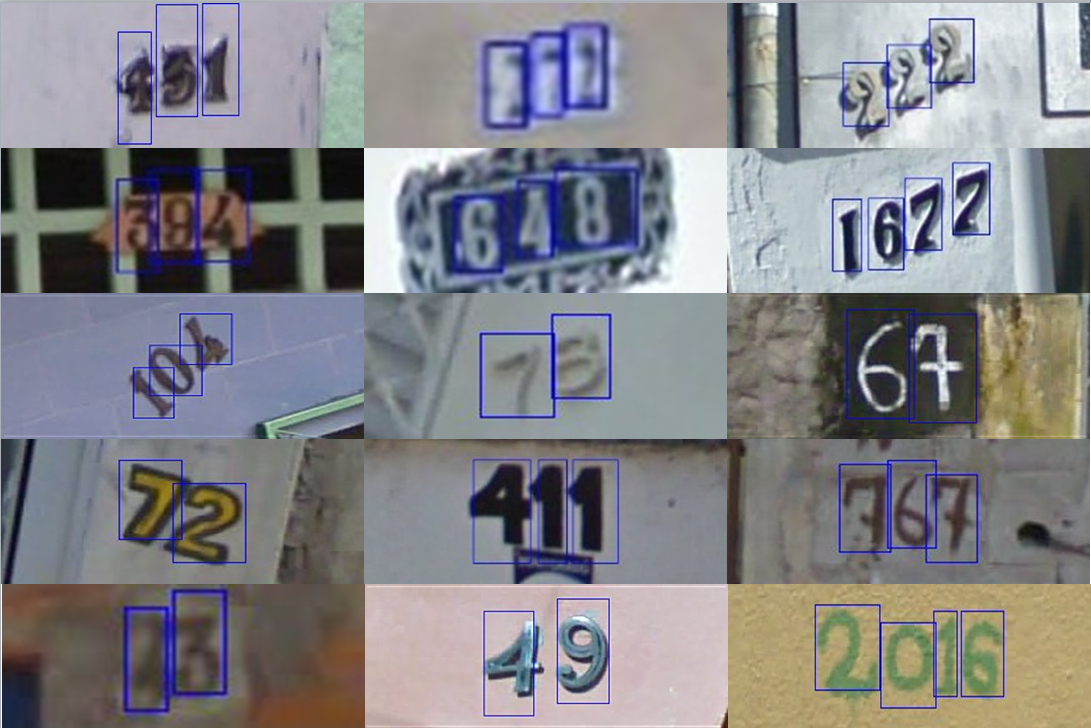
\includegraphics[width=1.0\textwidth, center]{svhn_numbers.png}
%  \end{center}
  \caption{SVHN Street Numbers}
  \label{fig:Fig4.1}
  \end{figure}
  
In the case of individual digit recognition, things were a bit more simple:
All images provided have dimensions of 32x32, and are (as in the previous case) coloured.
They originate from the numbers dataset used in the first part.
After being cropped from the images of the SVHN numbers dataset, the individual digit images are resized to 32x32, and used to 
create the digits dataset.
Therefore, no special preprocessing needs to be performed with regards to image size.
Like before, the digits dataset contains 10 classes, 1 for each digit. 
Digit '1' has label 1, '9' has label 9 and '0' has label 10.
Like previously, the labels are all one-hot-encoded during preprocessing, with the number of classes being 10 (one for each 
digit between 0 and 9). 
The distribution of the labels in the training and test dataset is displayed in figure \ref{fig:Fig4.2}.

\begin{figure}[H]
%\begin{center}
  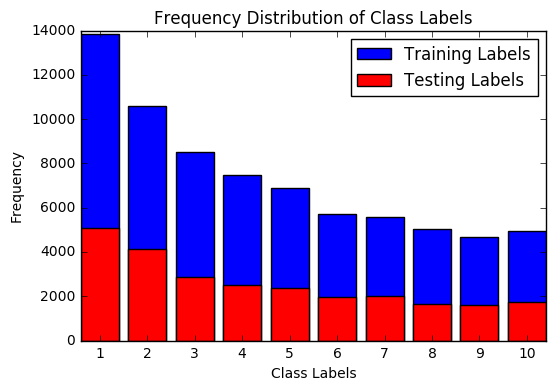
\includegraphics[width=1.0\textwidth, center]{distribution.png}
%  \end{center}
  \caption{Frequency Distribution of Class Labels}
  \label{fig:Fig4.2}
  \end{figure}
  
As can be seen, the data is not balanced, as digit 1 appears much more often than the rest.

\subsection{Algorithms and Techniques}
\label{sec:4.2}
As already discussed,in order to solve the problem, Deep Neural Networks were used, and more specifically 
Convolutional Neural Networks \cite{Fukushima1980} \cite{Lecun98gradient-basedlearning}.
Since the work consists of two parts, they will be discussed separately.

\subsubsection{Number recognition}
\label{sec:4.2.1}
In order to detect complete numbers, the model used initially 4 Convolutional Layers.
Convolutional layers are then followed by two fully connected layers.
There are 5 features predicted, each of them corresponding to one digit of the number we are trying to identify (0 was used as 
a 'no digit' indicator, in numbers that have length smaller than 5 (the maximum considered).
Therefore, there are 4 common Convolution Layers, and then two fully connected layers for each digit, with one output for 
each of the digits.

In order to solve the problem, that data was preprocessed.
Initially images were converted to grayscale, as they did not need to be coloured for the specific problem of number recognition.
This reduces significantly the size of our data.
Pixel values are then centered around zero, and they are normalised.
Images are cropped, discarding all other areas except the area that contains the number, which is derived from the  digit 
bounding boxes provided with the dataset.
Specifically, the bounding boxes for each digit are checked, and the points most to the left and the point most to the top
from the bounding boxes are identified.
Additionally, the points most to the right and the bottom are identified.
The area contained by the rectangle between these points is cropped from the original image.
It is then resized to 128x128, and replaces the original one in the dataset.

Finally, the labels are also processed, in order to conform with the design selected (length of five digits, 
zeros denoting the absence of a value).
Approximately 9\% of the original training set is used as validation set.
The models are created and trained using python \cite{python} and tensorflow \cite{45166}

The base model includes four convolution layers with stride one, followed by max pooling, and then two fully connected layers.
The optimiser used is Adam.
In the initial configuration (used as a baseline) Stochastic Gradient Descent was used, however then an Adam optimiser was 
selected, as we do not need to manually adapt the learning rate for different parameters.
The optimiser performs larger updates for infrequent, and smaller updates for frequent parameters.

The cost function used is softmax\_cross\_entropy\_with\_logits, included in the Tensorflow library.
Other configurations that will be tested include the use of dropout \cite{Srivastava2014} after the convolution layer, and for 
some after the hidden layer, and some also a decay of the learning rate.

The first step was to pre-process the data.
The images were processed, as well as the data available with them.
Included in the data were the label for each image, as well as the data defining the bounding box, in which the digits in each image can be found.

Initially, images were scaled down, so that calculations needed to be performed only over a more limited amount of pixels.
RGB images were be converted to grayscale, as colour information does not affect the identification of the digits themselves.
Converting the image to grayscale will allowed working on arrays with fewer dimensions.

As already mentioned, the dimensions of the data throughout the dataset varied.
Thus, the next step was to first select and crop the area defined as bounding box for each image, so we would work with the relevant information.
The images were cropped, so we can keep only this part.

Next, the image data was centred around zero, and normalized.
After that, the dataset was created, creating a list for each image with the labels in order, from the most significant, to the least significant digit.
90\% of the 'train' data was used as a training dataset, and the remaining was used as a validation dataset, as already mentioned.
the complete dataset was stored in python dictionaries, having different key-value pairs for image data and labels, for both the training, validation, and test set.
Then, they were stored altogether in a file, so that they can be reused multiple times, and the preprocessing process does not need to be repeated.

Regarding the actual neural network, there were two basic structures tested:
Initially, a setup consisting of a simple regression, where there are just the inputs and the outputs was tested, in order to use as a benchmark.
Then, a Convolutional Neural Network was created, which consisted of four convolution layers, followed by two fully connected layers.
The number of neurons in the hidden layer was initially 1024.
The network was trained using two different values for the number of training instances, with a batch of data of size 32, used as input during each training instance.
The Adam optimizer was used, with initially a steady learning rate of 1e-4.
The final Fully Connected layers are different for each one of the digits.
The effect of using dropout, or choosing different network parameters was studied, and the results from the different versions that were tested , were compared.

The cost function used was softmax\_cross\_entropy\_with\_logits, included in the Tensorflow library.
The models were created and trained using python \cite{python} and tensorflow \cite{45166}.
Weight initialisation was performed using the tensorflow truncated\_normal distribution with a standard deviation of 0.1.
Biases were initialized to zero.
Convolutions had a stride of 1, while for padding "SAME" was used, meaning the dimensions of the activation map for each layer were the same as the input.

After the last convolution layer, a max pooling operation was used, reducing the output dimension in half.
The size of the processed images used was initially chosen to be 128x128 pixels.

The steps taken during the project implementation were the following:

\begin{itemize}
\item The convolutional network was trained for 10000 steps.
\item Then, the same network was trained for 40000 steps.
\item The number of neuron in the hidden layer was reduced to 500, and dropout was added after the pooling operation, with keep probability of 0.6.
\item Then, the keep probability of the dropout was increased to 0.9.
\item Next, a learning rate decay was introduced, with the initial learning rate set to 0.5, and a reduction inversely analogous to the number of training steps, or \emph{epochs}.
\item Following that, a second dropout function was included after the hidden layer.
\end {itemize}


After that, some of the configurations were tested once again, this time using images of size 64x64.
the configurations used were the following:

\begin{itemize}
\item Double dropout with a learning decay, with initial learning rate 0.01, and keep probability 0.9, trained for 40000 steps.
\item Double dropout with a learning decay, with initial learning rate 0.5, and keep probability 0.9, trained for 40000 steps.
\item Double dropout without a learning decay, with learning rate  of 0.001, trained for 30000 steps.
\end {itemize}

Finally, the number of the hidden layers was reduced to 250, and a configuration with double dropout without learning decay, 
with learning rate of 0.01, was tested, after being trained for 40000 steps.
The various configurations are summarised in table \ref{tab:Table 4.1}, where probability refers to the probability of keeping an input.

\begin{table}[H]
\caption{Network configurations used.}
\centering
\begin{tabular}{ c  c  c  c  c  c  c }
\hline
Configuration& Optimizer &Number of     & Dropout & Learning  & Training & Image\\
      No     &           &Hidden Nodes  &         & rate      & Steps    & Dimensions\\
		 
\hline
1&GradientDescent&500&No&0.5&40,000&128x128\\
%\hline
2&AdamOptimizer&1024&No&1e-4&10,000&128x128\\
%\hline
3&AdamOptimizer&1024&No&1e-4&40,000&128x128\\
%\hline
4&AdamOptimizer&500&Once, Prob.:0.6&1e-4&40,000&128x128\\
%\hline
5&AdamOptimizer&500&Once, Prob.:0.9&1e-4&40,000&128x128\\
%\hline
6&AdamOptimizer&500&Twice, Prob.:0.9&1e-4&40,000&128x128\\
%\hline
7&AdamOptimizer&500&Once, Prob.:0.9&1e-2/decay&40,000&128x128\\
%\hline
8&AdamOptimizer&500&Twice, Prob.:0.9&1e-2/decay&40,000&64x64\\
%\hline
9&AdamOptimizer&500&Twice, Prob.:0.9&0.5/decay&40,000&64x64\\
%\hline
10&AdamOptimizer&500&Twice, Prob.:0.9&1e-2&30,000&64x64\\
%\hline
11&AdamOptimizer&250&Twice, Prob.:0.9&1e-2&40,000&64x64\\
\hline
\end{tabular}
\label{tab:Table 4.1}
\end{table}

\subsubsection{Digit recognition}
\label{sec:4.2.2}
In the second part of the work, the aim was to identify individual digits.
Since the image size was smaller this time, and there was only one output, the model was much simpler.

This time, there were 3 Convolution Layers, followed again by 2 fully connected layers.
There is one feature predicted, which is the digit to be identified.
Classes are 10, one for each digit between 0 and 9.
As already mentioned, the labels are all one-hot-encoded during preprocessing

Besides that, preprocessing included centering pixel values around zero, and normalising them.
Additionally, the shape of the data was changed, from (img_length, img_width, num_channels, num_images), to 
(num_images, img_length, img_width, num_channels), for simpler processing.

Same as in the first part of the work (number recognition), approximately 9\% of the original training set is used as 
validation set.
The models are - like before - created and trained using python \cite{python} and tensorflow \cite{45166}

The base model includes three convolution layers with stride one, each followed by a relu unit, and max pooling with stride 2, 
which has padding "VALID".
Then, follow two fully connected layers.
After the first fully connected layer, dropout \cite{Srivastava2014} is also used, in order to prevent over-fitting.
The keep probability used was 0.9.
The optimiser used is once again Adam.


The cost function used is like in the number recognition case,  softmax\_cross\_entropy\_with\_logits, included in the 
Tensorflow library.


Regarding the actual neural network, there were two basic structures tested:
Initially, a setup consisting of a simple regression, where there are just the inputs and the outputs was tested, in order to use as a benchmark.
Then, a Convolutional Neural Network was created, which consisted of four convolution layers, followed by two fully connected layers.
The number of neurons in the hidden layer was initially 1024.
The network was trained using two different values for the number of training instances, with a batch of data of size 32, used as input during each training instance.
The Adam optimizer was used, with initially a steady learning rate of 1e-4.
The final Fully Connected layers are different for each one of the digits.
The effect of using dropout, or choosing different network parameters was studied, and the results from the different versions that were tested , were compared.

The cost function used was softmax\_cross\_entropy\_with\_logits, included in the Tensorflow library.
The models were created and trained using python \cite{python} and tensorflow \cite{45166}.
Weight initialisation was performed using the tensorflow truncated\_normal distribution with a standard deviation of 0.1.
Biases were initialized to zero.
The network was then trained for 240001 steps, and finally used on the test set.
A graphical representation of the model used, where the dimensions of the output of each layer are displayed, can be found in 
figure \ref{fig:Fig4.3}.

\begin{figure}[H]
%\begin{center}
  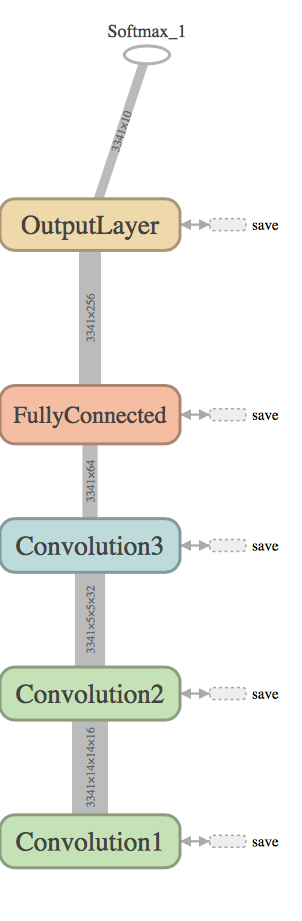
\includegraphics[width=1.0\textwidth, center]{network.png}
%  \end{center}
  \caption{Model Structure Used for Digit Recognition}
  \label{fig:Fig4.3}
  \end{figure}
  


\subsection{Benchmark Model}
\label{sec:4.3}
The Benchmark for the number recognition application was the naive model, where we only have the inputs, and regression outputs.
Efficiency criterion was the detection accuracy.
The accuracy is defined as described in chapter \ref{sec:3.2}.
The various configurations used were examined, and compared to our naive model (in this case, a simple regression model).
In the case of individual digit recognition, there are many implementations, therefore it is much easier to find a benchmark.
The goal for digit recognition is to achieve an accuracy comparable to - or not dramatically worse than
the one achieved by the configuration of the authors of \cite{DBLP:journals/corr/GoodfellowBIAS13} used (96.03\% for sequence transcription), 
or that of humans (98\%).
In any case, an accuracy of around 90\% on the test set, would be an acceptable result from the model.


 
\section{Results}
\label{sec:5}
\subsection{Model Evaluation and Validation}
\label{sec:5.1}
\subsection{Number Recognition}
\label{sec:5.1.1}
As can be seen in figure \ref{fig:Fig5.1}, The accuracy of the naive model that was used as baseline (the simple model using regression) 
had a prediction accuracy that was only 0.7\%.
The model was underfitting the data, as the accuracy measured on the training set was also very low, at most around 10\%.
Using the model with the convolutions and the fully connected layers previously described, resulted in a significant increase of the accuracy up to 10,000 epochs, 
and a smaller one when training continued up to 40,000 steps, reaching 37\%.
However, the model was clearly overfitting the data, since the training set accuracy reached levels of 100\%.
Configuration No 4, introduced dropout, with a keep probability of 0.6.
In addition, the number of hidden nodes were reduced to 500.
This produced a model that had a very low accuracy on the test set (2.9\%) and a bit higher on the training set, but not significantly.

The highest accuracy observed was when the keep probability of the dropout was increased to 0.9, and then a second dropout function was introduced (configurations 5,6).
The model with double dropout had an accuracy of 47.7\% on the test set, while the one with the single dropout slightly less.
Both of them though were still overfitting the data, since their training accuracy reached 100\%.
Introducing a learning rate decay reduced significantly accuraxy to 2.4\%.

Reducing the dimensions of the input image to 64x64 did not yield better results: the contrary.
The accuracy of models 8-11 did not exceed 13.7\% (Configuration No 11, the one without a learning rate decay).
In cases 7-10 it was around 2.5\%, and once again underfitting the data. 

The situation seemed to improve a bit when the number of hidden neurons was reduced to 250, however the results were still far from 
those witnessed with configurations 5 and 6.


\begin{figure}[H]
%\begin{center}
  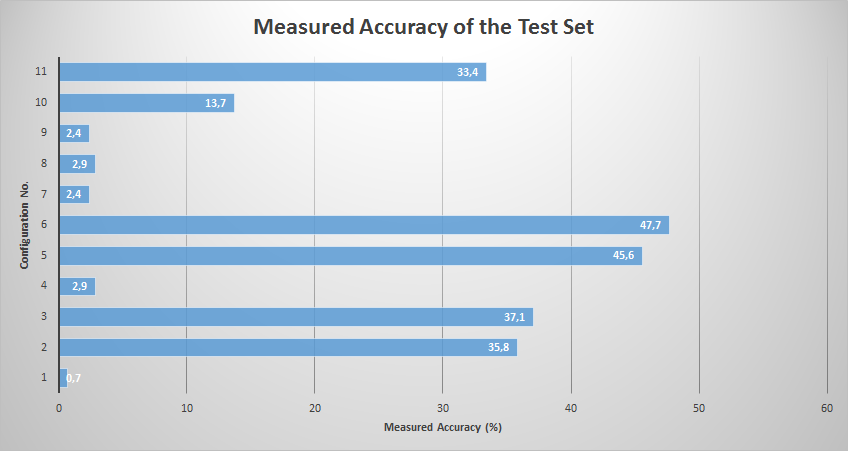
\includegraphics[width=1.0\textwidth, center]{accuracy.png}
%  \end{center}
  \caption{Test Set Accuracy}
  \label{fig:Fig5.1}
  \end{figure}

\subsection{Digit Recognition}
\label{sec:5.1.2}
The model was trained for 240001 steps.
Data was fed to the network in batches of 128 at the time.
As can be seen in figure \ref{fig:Fig5.2}, the accuracy of each minibatch was increasing, reaching in the end ..\%.
At the same time, the cost was decreasing, as is displayed in figure \ref{fig:Fig5.3}.
The accuracy on the validation set was also monitored during the training process.
It was also increasing as the network was training, reaching eventually ..\%.
A graphical representation of the accuracy on the validation set can be seen in figure \ref{fig:Fig5.4}.


\begin{figure}[H]
%\begin{center}
  \includegraphics[width=1.0\textwidth, center]{batch.png}
%  \end{center}
  \caption{Accuracy of Training Set Batches Prediction}
  \label{fig:Fig5.2}
  \end{figure}
  
  \begin{figure}[H]
%\begin{center}
  \includegraphics[width=1.0\textwidth, center]{batch.png}
%  \end{center}
  \caption{Cost Value During Network Training}
  \label{fig:Fig5.3}
  \end{figure}


\begin{figure}[H]
%\begin{center}
  \includegraphics[width=1.0\textwidth, center]{batch.png}
%  \end{center}
  \caption{Accuracy of Prediction of Validation Set}
  \label{fig:Fig5.4}
  \end{figure}
  
Finally, when attempting to identify the digits of the test set, the model had a prediction accuracy of 0.7\%.





\section{Discussion and Future Work}
\label{sec:6}
\subsection{Number Recognition}
\label{sec:6.1}
As can be deducted from the results presented above, the solution selected, with the for convolution layers and the 
two fully connected layers, can provide results that may not be comparable to the state of the art, however are significantly 
superior to the naive approach used as benchmark.
This of course, provided the right hyperparameters are selected, like the number of hidden nodes, dropout keep probability, etc.

Most of the state of the art solutions study digit recognition.
Therefore, there are not many solutions to compare with.
In any case, An accuracy around 50\% is considered low.
In the environment where the tests took place, adding more layers would not be efficient, since the processing power of the system used is limited.
Even The currently tested architectures took at least a couple of days to train each, depending on the number of steps, as well as image size, etc.
Therefore, even though testing architectures with more layers would be interesting in order to compare results with the 
architectures currently used,  the required time for performing all tests would range from weeks to months 
(using the hardware used).

However, perhaps the most important reason for the low accuracy, is the way the model is structured, with a fixed number of 
digits for each number.
Identifying the "no digit" in an image is probably difficult, especially in an image that is cropped, and contains only the 
actual digits.
A solution where the labels would have varying length (up to 5), and the length of each number was identified together with 
the digits, would probably yield better results.
This, however, needs to be examined with a future version of the model.

Another direction to be pursued in the future is to perform the same tests, using the same models, only this time using the 
original images. Meaning, instead of cropping the SVHN images and keeping only the parts contained in the provided bounding boxes, 
to use the complete provided images.
A final step would be to use the original images, and simultaneously try to output the bounding boxes, besides the digits in the images 
themselves.

However, the most useful probably adjustment would be just detecting digits using the original images, and adjust the implementation, 
so that real time video can also be used.
This can then find many applications, for example be used in systems like autonomous vehicles, in order to identify road signs, 
or detect in real time licence plates of cars, etc.
\subsection{Digit Recognition}
\label{sec:6.2}
As can be deducted from the results presented above, the solution selected, with the for convolution layers and the 
two fully connected layers, can provide results that may not be comparable to the state of the art, however are significantly 
superior to the naive approach used as benchmark.
This of course, provided the right hyperparameters are selected, like the number of hidden nodes, dropout keep probability, etc.

The state of the art solutions that provide accuracy comparable to that of the human, have mostly many more layers than the models tested.
In the environment where the tests took place, adding more layers would not be efficient, since the processing power of the system used is limited.
Even the currently tested architectures took at least a couple of days to train each, depending on the number of steps, as well as image size, etc.
Therefore, even though testing architectures with more layers would be interesting in order to compare results with the ones currently used, 
the required time for performing all tests would range from weeks to months (using the hardware used).

A second direction to be pursued in the future is to perform the same tests, using the same models, only this time using the 
original images. Meaning, instead of cropping the SVHN images and keeping only the parts contained in the provided bounding boxes, 
to use the complete provided images.
A final step would be to use the original images, and simultaneously try to output the bounding boxes, besides the digits in the images 
themselves.

However, the most useful probably adjustment would be just detecting digits using the original images, and adjust the implementation, 
so that real time video can also be used.
This can then find many applications, for example be used in systems like autonomous vehicles, in order to identify road signs, 
or detect in real time licence plates of cars, etc.


\section{Conclusion}
\label{sec:6.3}
As has been described above, an attempt was made to identify digits and complete numbers, from images in the Street View House 
Numbers dataset.
The dataset images, along with the labels were obtained, and imported to the python application developed.
Then, they were preprocessed, image pixel values centered around zero and normalised, and labels one-hot-encoded.
(In the case of number recognition, additionally processed in order to reflect the complete number)

Then, the network consisting of convolution layers with relu activations and max pooling was trained, and the output was generated 
through two fully connected layers.
The accuracy was studied for various configurations in the case of number detection, and a configuration similar to the one 
that produced the highest accuracy with number recognition, was also used to study individual digit recognition.

The results have been discussed in sections \ref{sec:5.1.1} and \ref{sec:5.1.2}.

One improvement in both cases could be the use of better hardware, that makes use of GPUs, in order to speed up computations.
This would allow for testin of more configurations/different models.
Furthermore, it would enable the use of more training data, as the time required for the model to process them would be significantly reduced.

One additional thing that would definitely help would be to use data augmentation techniques, in order to generate additional data.
This is expected to be extremely important, especially in the case of the models that are overfitting the data.
Since the models that displayed the best results on the test data were actually overfitting, the use of additional data is expected 
to improve the accuracy of the model further.
Such techniques have been explored, and it is planned as a next step to use functions that are built in scikit-learn and tensorflow, in 
order to create further data, and examine if the accuracy of the test set predictions will be improved, and to what extend.
What is used in future versions of the number recognition program developed, are functions from the from PIL python package, 
and more specifically , the PIL ImageFilter EMBOSS, BLUR, CONTOUR, SMOOTH_MORE, and SHARPEN filters.
These are used to create five more training datasets, with the images slightly distorted, which can be used in conjunction with 
the original one, to train the model further.



\clearpage

\bibliographystyle{elsarticle-num}
\bibliography{mybibliography}



\end{document}